\documentclass[12pt, letterpaper]{article}
\usepackage[utf8]{inputenc}
\usepackage[letterpaper, margin=3.cm]{geometry}
\usepackage{graphicx}
\graphicspath{{/home/clebson/Documents/ComplexNetworksDCC/tp3/img//}}

\usepackage{epstopdf}
\epstopdfsetup{outdir=./}


\title{Experimento com NetLogo}
\author{Clebson C. A. de Sá}

\begin{document}
\maketitle

\section{Small World}
A primeira questão pede para considerar o modelo ``Small-World``.
A análise consistiu em uma rede baseada em 40 nós, no qual uma série de experimentos
foram realizados no software NetLogo com o intuíto de entender as características 
da rede.
A primeira observação a ser feita é que as conexões de cada nó levam em 
consideração a probabilidade de conexão entre os nós. No programa é possível
indicar a probabilidade que deseja avaliar por meio da variação do 
parâmetro ``rewiring-probability''.
As ligações são aleatoriamente proporcionais a esta probabilidade. Assim sendo,
para se ter uma boa estimativa deste parâmetro torna-se necessário efetuar repetições 
do experimento para computar o desvio padrão e entender melhor a variação em relação
a média. Para capturar esta informação foram executados 10 repetições para cada variação do parâmetro 
``rewiring-probability'' considerando o intervalo de $\left[0.1, 0.9\right]$ com
intercalação de $0.1$.
Os resultados para este experimento podem ser visualizados na Figura \ref{fig:small-world}
para ambas as métricas avaliadas com o devido desvio padrão.

\begin{figure*}[h]
  \centering
  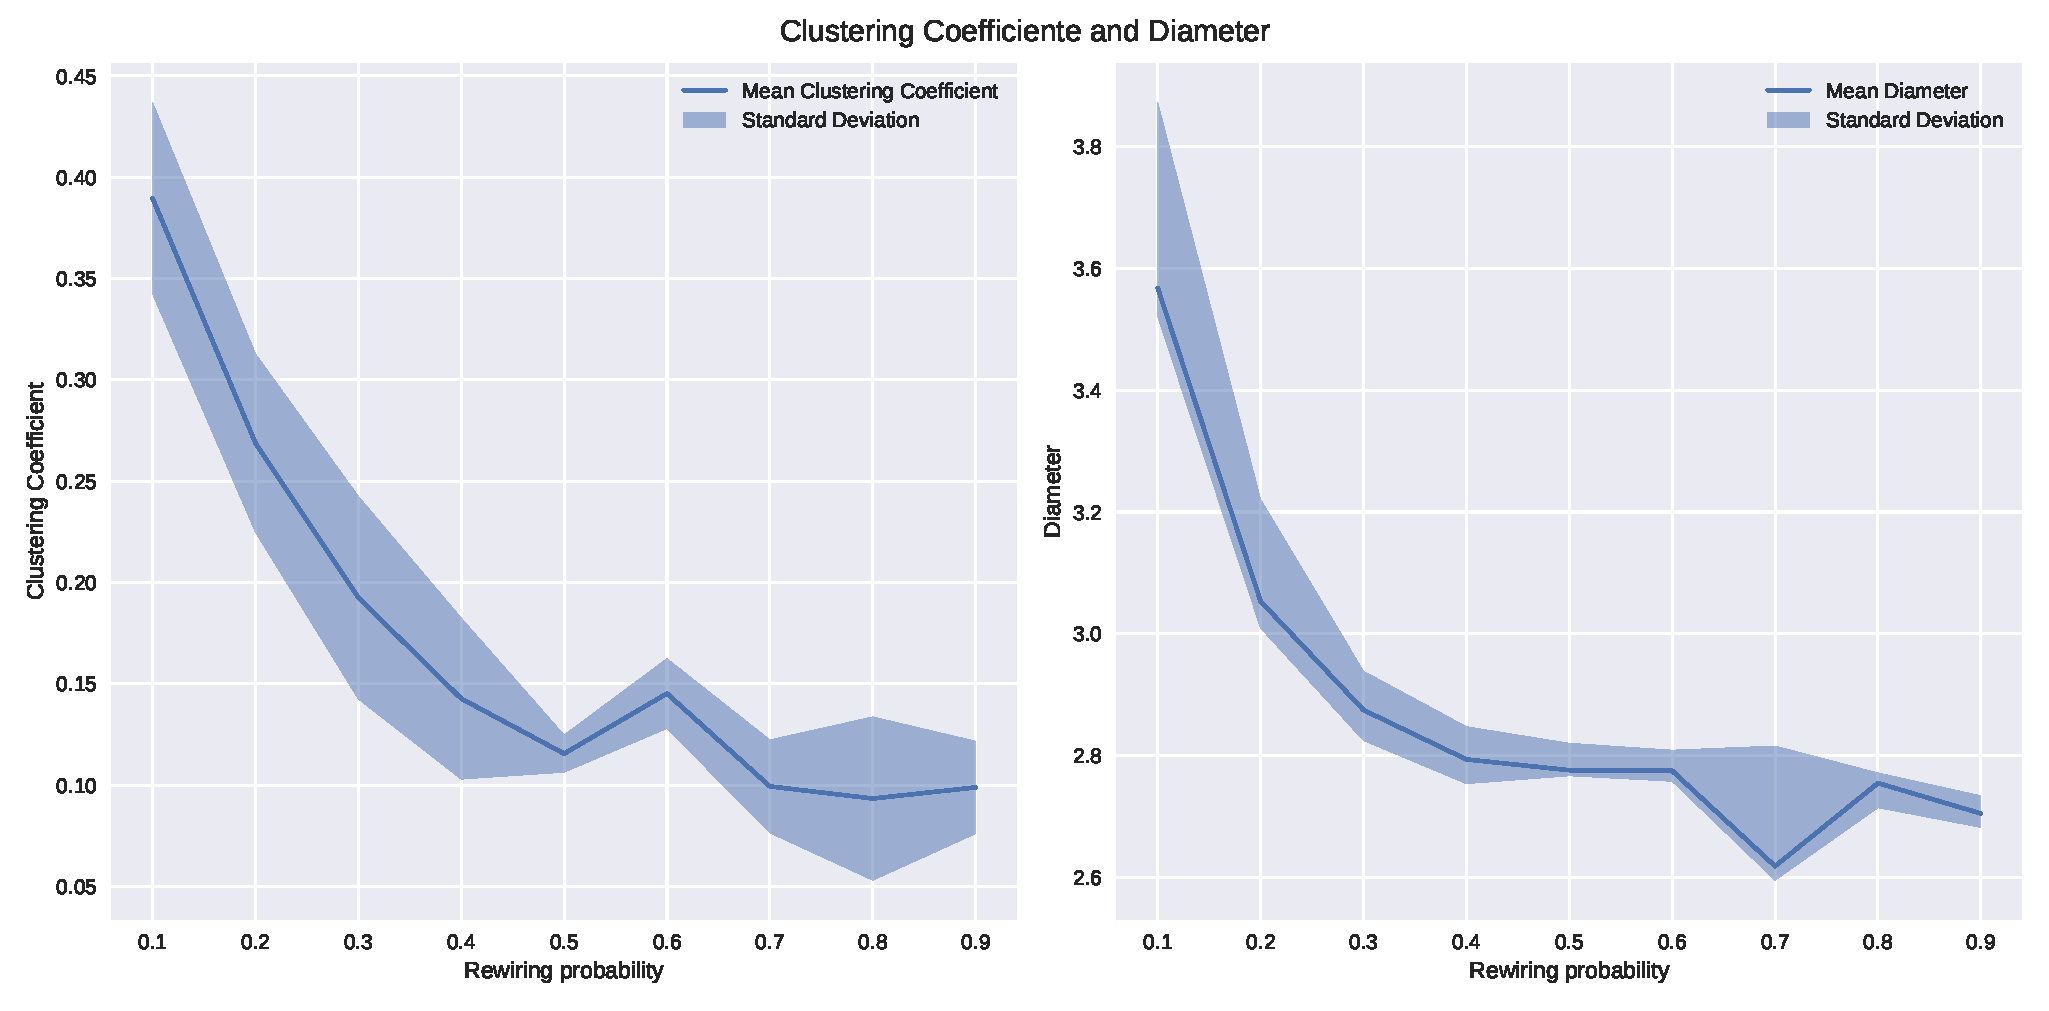
\includegraphics[scale=0.4]{graphProb1.pdf}
  \caption{Coeficiente de Clusterização e Diâmetro com variação da probabilidade.}
  \label{fig:small-world}
\end{figure*}


Conforme podemos visualizar nesta figura, os valores para o Coeficiente de Clusterização
e Diâmetro diminuem conforme aumenta-se a probabilidade de linkagem entre os nós.
Isto é também confirmado ao observar o coeficiente de correlação Pearson de $0.88$
considerando todas as amostras do experimento conforme mostrado na Figura \ref{fig:correlation}.

\begin{figure*}[h]
  \centering
  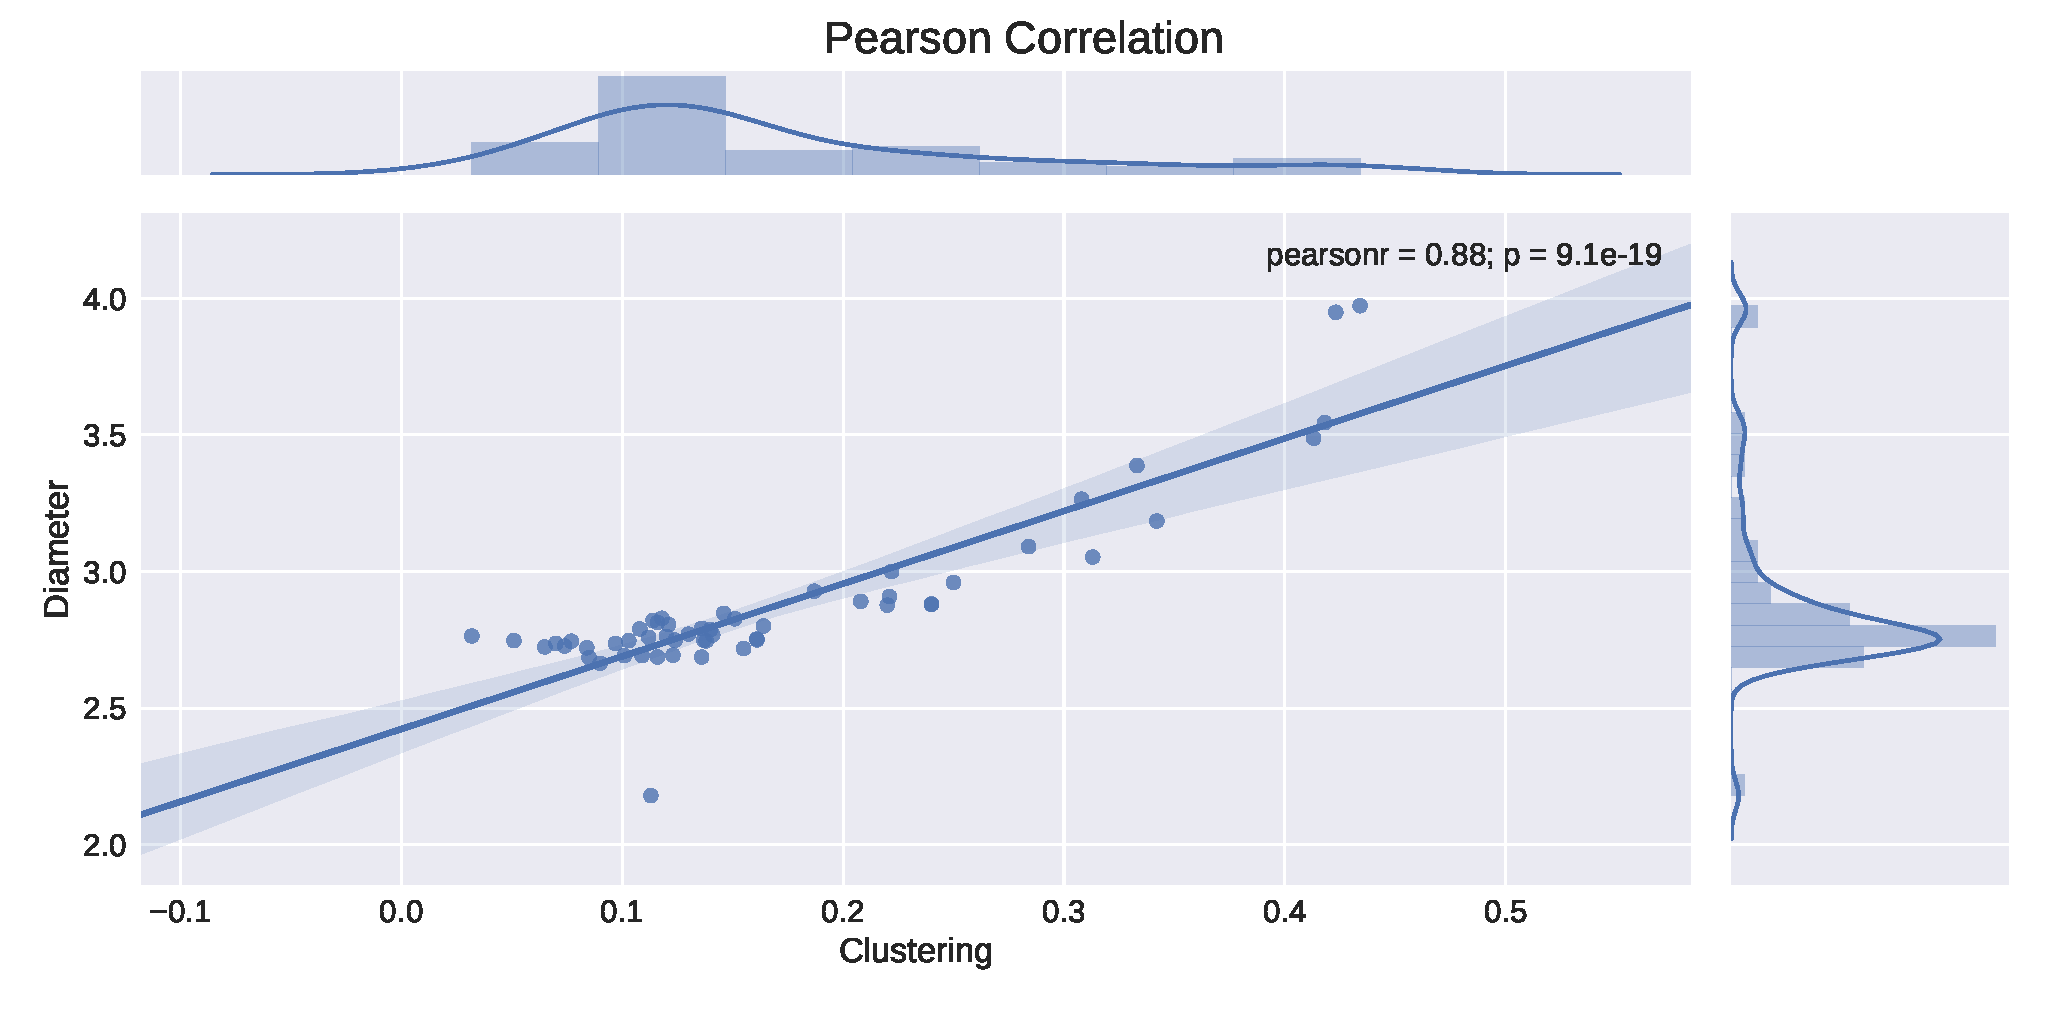
\includegraphics[width=1\textwidth]{graphCorrelation.pdf}
  \caption{Correlação de Pearson com Regressão Linear das métricas avaliadas.}
  \label{fig:correlation}
\end{figure*}

Ainda nesta Figura, podemos observar a distribuição de ambas as métricas
por meio do histograma em ambos os eixos. O histograma do  Coeficiente de 
Clusterização nos mostra que grande maioria dos valores observados estão espalhados
entre $\left[0.05, 0.15\right]$. Comparando este intervalo da distribuição de 
clusterização podemos explicar melhor o motivo do alto valor do desvio padrão 
na Figura \ref{fig:small-world} em torno da probabilidade $\left[0.7, 0.9\right]$.
Em relação à distribuição do Diâmetro podemos observar no histograma que a maior
parte dos valores observados estão entre o intervalo $\left[2.5, 3.0\right]$.

Podemos concluir que estes resultados de fato fazem sentido, visto que batem com
o conceito de Redes de mundo pequeno, visto que com o aumento da probabilidade
existe o aumento da quantidade de links  entre os nós. Logo podemos inferir os 
valores para quaisquer probabilidades por meio da regressão linear também mostrada
na Figura \ref{fig:correlation}.



\section{Aids}
Considerando os modelos de ciências sociais disponibilizado pelo Software Netlogo
foi feito a simulação de infecção do vírus HIV em um conjunto de 300 pessoas. Nesta
simulação está sendo considerado grupos de pessoas que tiveram relações sexuais
mutuamente no mesmo período de tempo sem nenhuma fonte de segurança como utilização
de preservativos.
Os resultados para este experimento podem ser visualizados na Figura \ref{fig:aids}.

\begin{figure*}
  \centering
  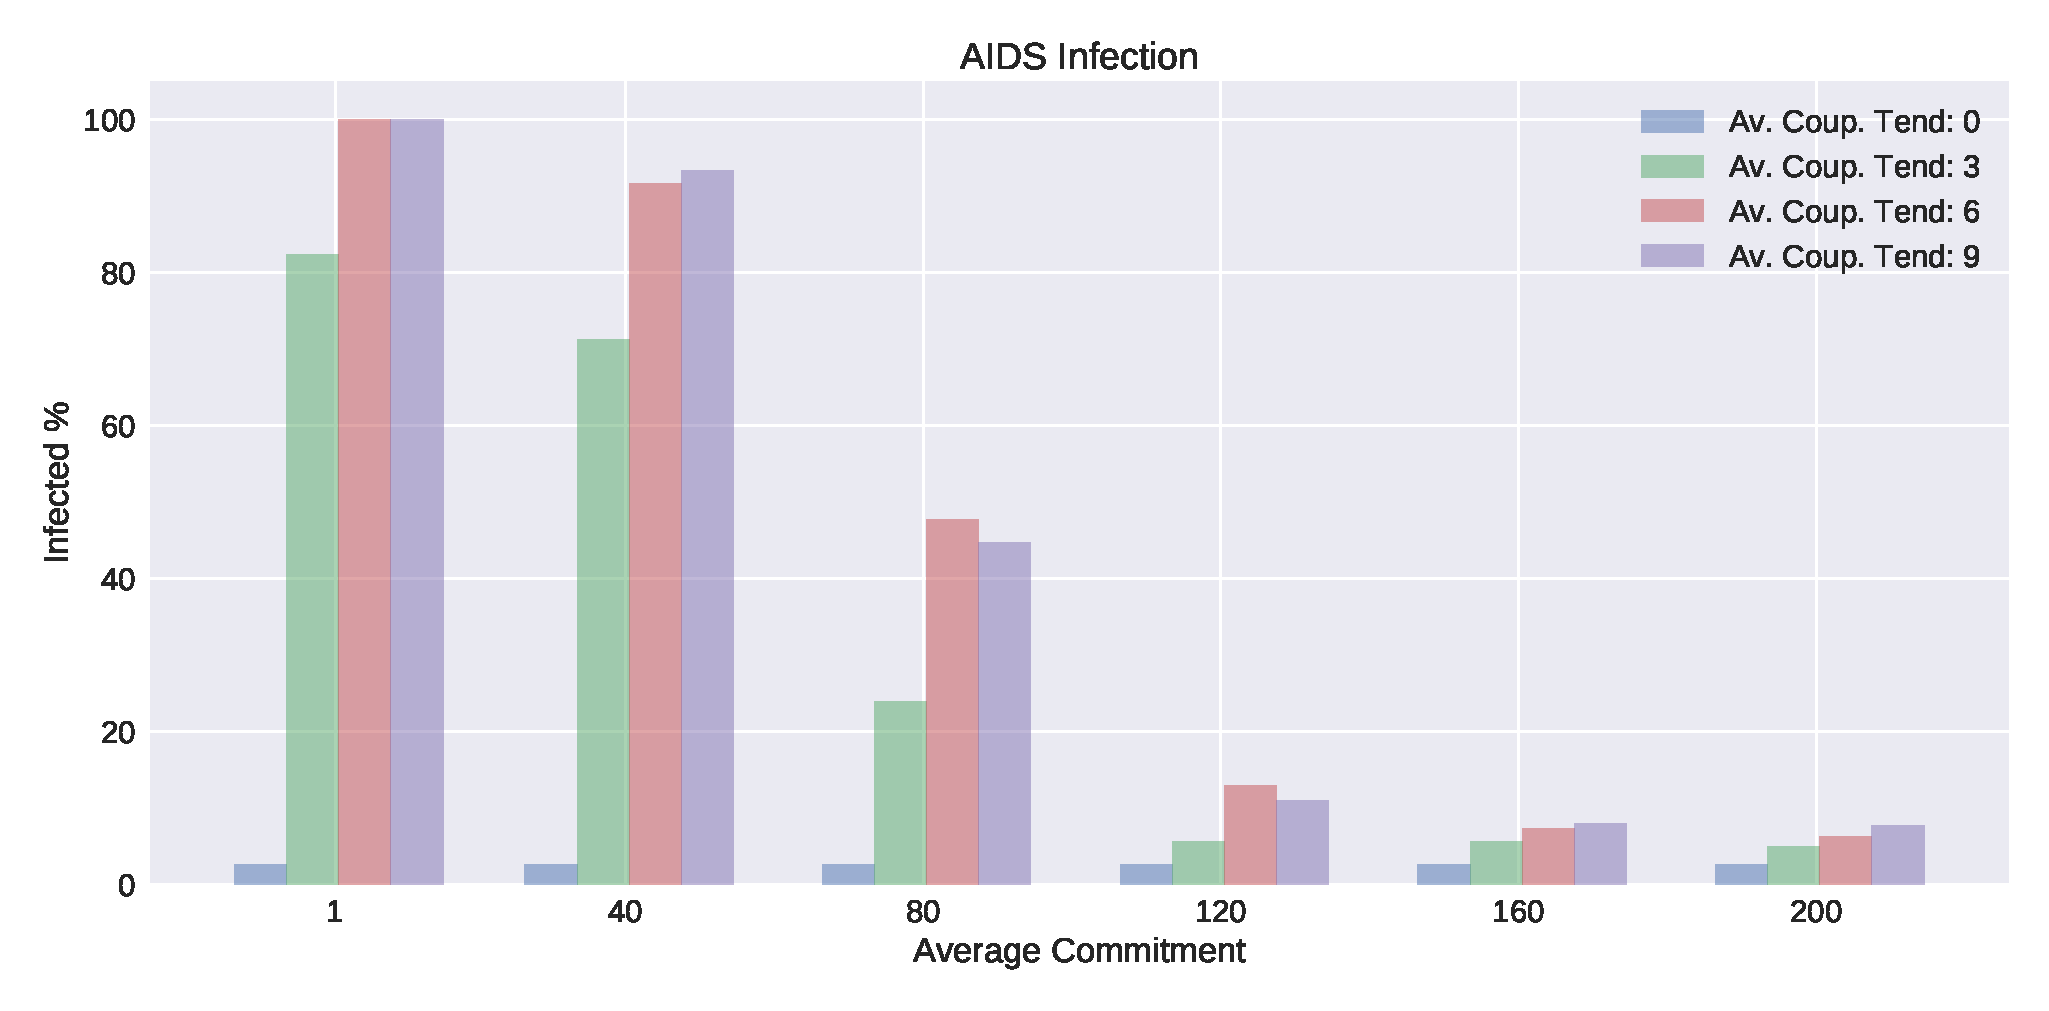
\includegraphics[width=1\textwidth]{aids.pdf}
  \caption{Simulação do vírus HIV}
  \label{fig:aids}
\end{figure*}

Conforme podemos visualizar nesta Figura, quando a quantidade de relações conjuntas
(i.e: parâmetro ``Av. Cup. Tend.'' no gráfico) são parametrizadas com 0 a porcentagem
de pessoas infectadas é de $\approx 2.67$ durante todo o período em que as relações
sexuais acontecem. Pode ser observado também nesta figura que conforme a quantidade
de relações em conjunto aumenta, a tendência é atingir o maior número de pessoas
infectadas nas semanas iniciais. Por exemplo, para o parâmetro ``Av. Coup. Tend.
6 e 9'' podemos observar que todas as pessoas são infectadas logo na primeira seamana.
Podemos concluir também que conforme as pessoas passam a ter tendências monogamicas
a porcentagem de infecção é bem menor. Como exemplo podemos citar a porcentagem
de infecções existentes no parâmetro ``Average Commitment 200'' que é abaixo
de $15\%$.




\end{document}
